\chapter{Preliminaries}

\label{fundamentals}

\pagenumbering{arabic}

A gaseous substance, ionised through a strong rise in temperature or by photo-ionization, whose constituent particles are predominantly electrons and ions of various species, yet whose density is sufficiently low for the constituent particles to follow the Maxwell distribution rather than that of Paul-Dirac or Bose-Einstein, is termed a \textit{plasma}. The differential equations governing plasma behaviour generally lack simple exact models, because the dynamics of the constituent particles intertwine delicately with their trajectories at any given instant. Furthermore, the overabundance of particles renders the search for exact solutions in practice infeasible. However, due to the same overabundance, statistical tools prove particularly useful, as they provide a simplified approach to describing plasma phenomena.

\section{Parameters and examples of plasma}

The three fundamental parameters that characterize plasmas are:

\begin{enumerate}
    \item The density $n$ of the constituent particles, measured in particles per cubic meter,
    \item The temperature $T$ of each species, often measured in eV (where $1\,\text{eV}=11\,605\,\text{K}$),
    \item The magnetic field $\mathbf{B}$ in steady state, expressed in teslas.
\end{enumerate}

Numerous additional parameters, such as the Debye length, the Larmor radius, and the thermal velocity of each species, among many others, are derived from these three main parameters. It is worth mentioning, as an exception, some remarkable peculiarities of partially ionized plasmas, where the dominant presence of neutral particles is of comparable relevance to that of charged particles.

\section{Logical scheme of plasma physics}

Plasmas exist within a wide range of conditions, spanning several orders of magnitude in each of the aforementioned quantities. Plasma physics cannot, in many cases, be considered an exact science; rather, it comprises numerous regimes and associated models grounded in well-justified conditions and approximations, each designed to describe a limited range of situations. In this first introductory chapter to plasma physics, we focus on expanding and deepening our understanding of plasma dynamics. Our study of plasma physics will adopt a selective focus on specific viewpoints in plasma dynamics, while preserving a global perspective that connects them into a coherent network of plasma phenomena. Plasma dynamics is primarily determined by the interaction between electromagnetic fields and the motion of constituent particles. From a pragmatic statistical perspective, the latter are considered to be present in very large numbers. Assuming time were not a constraint and measurement precision were absolute, the evolution of any form of plasma could be modelled according to the following procedure:

\begin{enumerate}
    \item Given the trajectory $\mathbf{x}_i(t)$ and velocity $\mathbf{v}_i(t)$ of any particle, the electric field $\mathbf{E}(\mathbf{x},t)$ and magnetic field $\mathbf{B}(\mathbf{x},t)$ can be evaluated using Maxwell's equations.
    \item Given the \textit{instantaneous} electric and magnetic fields $\mathbf{E}(\mathbf{x},t)$ and $\mathbf{B}(\mathbf{x},t)$, the forces acting on any particle can be evaluated using the Lorentz equation to update their trajectories and velocities.
\end{enumerate}

However, such procedures are not practicable given the very large number of particles and, to a lesser extent, the complexity of the electromagnetic field. To achieve a more practical understanding, we will abandon the precise evaluation of complex behaviour in its entirety and restrict our considerations to specific phenomena within a given regime. A \textit{regime} is a situation in which certain approximations remain relevant and allow for a system's coherent description. The following categories of approximations allow us to establish numerous regimes:

\begin{enumerate}
    \item Approximations concerning the electromagnetic field:
    \begin{enumerate}
        \item Assumption of the absence of a magnetic field (unmagnetised plasma);
        \item Assumption of the absence of inductive fields (electrostatic approximation);
        \item Neglect of the displacement current in Ampère's law (applicable to phenomena where certain characteristic speeds are much smaller than the speed of light);
        \item Assumption that any magnetic field originates from an external conductor;
        \item Assumptions concerning the geometry of the system (existence of symmetries, uniformity).
    \end{enumerate}
    \item Approximations concerning particle properties:
    \begin{enumerate}
        \item Considerations on the Lorentz force acting on certain groups of particles:
        \begin{enumerate}
            \item Using a distribution function $f_\sigma(\mathbf{x}, \mathbf{v}, t)$ of a species $\sigma$ whose velocity is $\mathbf{v}$ at position $\mathbf{x}$ at time $t$ (Vlasov theory).
            \item By taking the average of the velocities of all particles of species $\sigma$ located in the vicinity of $\mathbf{x}$, and characterizing, using the density $n_\sigma(\mathbf{x}, t)$, the mean velocity $\mathbf{u}_\sigma(\mathbf{x}, t)$ and the pressure of the species $P_\sigma(\mathbf{x}, t)$ (two-fluid theory).
            \item By taking the average of the momenta of all particles of any species and characterizing the plasma by the centre-of-mass density $\rho(\mathbf{x},t)$, the centre-of-mass velocity $\mathbf{U}(\mathbf{x}, t)$, and the pressure $P(\mathbf{x}, t)$ defined relative to the centre-of-mass velocity $\mathbf{U}(\mathbf{x}, t)$ (magnetohydrodynamic theory).
        \end{enumerate}
        \item Assumptions concerning time (that the frequency of the considered phenomenon is lower or higher than certain characteristic frequencies of the plasma);
        \item Assumptions concerning space and its dimensions (that the domain of influence of the considered phenomenon is larger or smaller than certain characteristic lengths of the plasma);
        \item Assumptions concerning particle velocities (that the phenomenon spreads more or less quickly than the thermal speed of species $\sigma$).
    \end{enumerate}
\end{enumerate}

If we consider the approximations listed above again, we will not necessarily see a structured hierarchy. Unfortunately, developing an intuition first requires admitting some of these approximations. This leaves us uncertain about how to approach the subject, as we must accept certain concepts on faith that their results will be valid, in the hope of later affirming their validity. Consequently, it will be necessary to consult the following scheme from time to time:

\begin{figure}[H]
    \centering
    \scalebox{0.8}{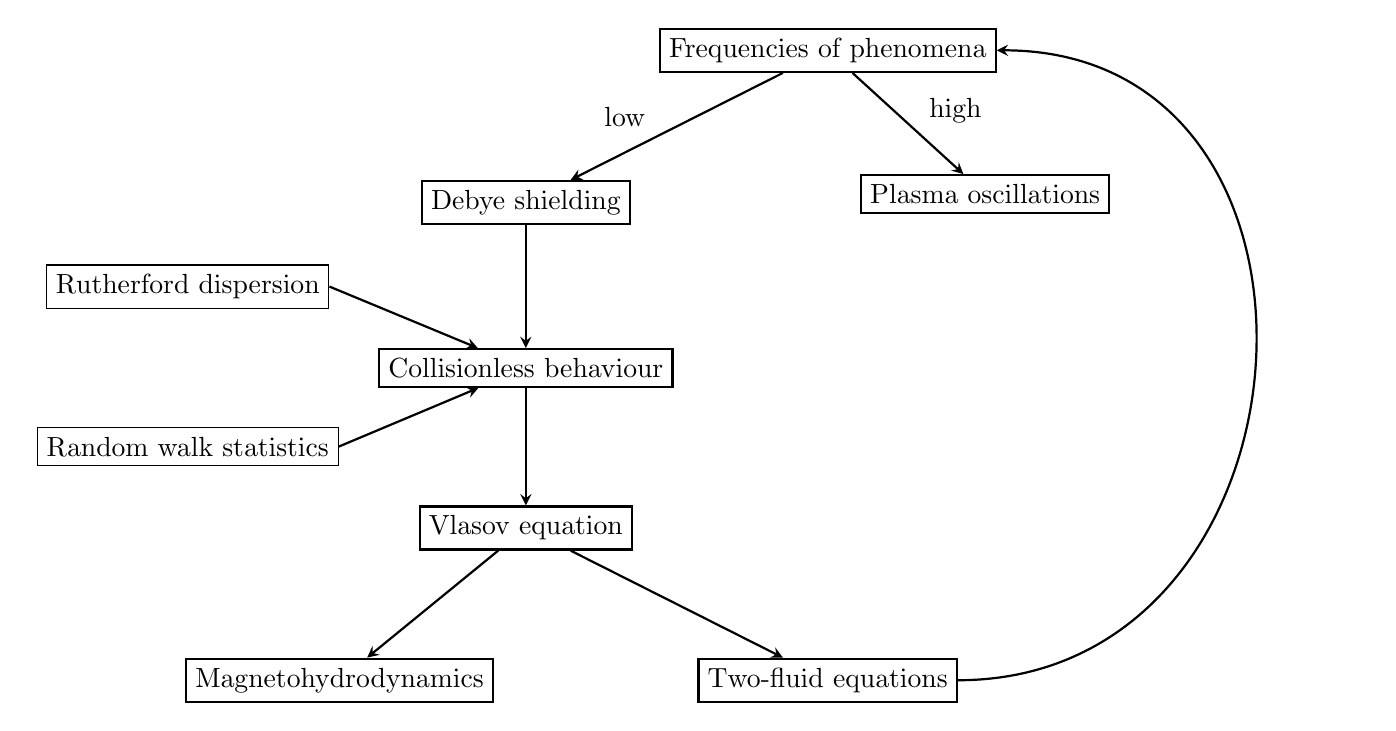
\begin{tikzpicture}[scale=1, every text node part/.style={align=center}, auto, line/.style ={draw, thick, -latex',shorten >=2pt}]
    \coordinate (freq) at (6, 4);
    \node[draw, thick] (frfr) at (freq) {Frequencies of phenomena};
    \coordinate (wifi) at (8, 2.175);
    \node[draw, thick] (hifi) at (wifi) {Plasma oscillations};
    \matrix[row sep=0.5cm,column sep=0.5cm] {
        & \node[draw, thick] (Debye) {Debye shielding}; \\
        \node[draw] (Ruth) {Rutherford dispersion}; & \\
        & \node[draw, thick] (Plas) {Collisionless behaviour}; \\
        \node[draw] (Walk) {Random walk statistics}; & \\
        & \node[draw, thick] (Vlas) {Vlasov equation}; \\
    };
    \draw[thick, -stealth] (Debye) -- (Plas);
    \draw[thick, -stealth] (Ruth.east) -- (Plas);
    \draw[thick, -stealth] (Walk.east) -- (Plas);
    \draw[thick, -stealth] (Plas) -- (Vlas);
    \coordinate (MHD) at (-0.2, -4);
    \coordinate (2F) at (6, -4);
    \node[draw, thick] (mhd) at (MHD) {Magnetohydrodynamics};
    \node[draw, thick] (2f) at (2F) {Two-fluid equations};
    \draw[thick, -stealth] (Vlas) -- (mhd);
    \draw[thick, -stealth] (Vlas) -- (2f);
    \coordinate (aux) at (7, 3.5);
    \draw[thick, -stealth] (2f.east) to[out=0, in=0, looseness=1.5] (frfr.east);
    \draw[thick, -stealth] (frfr) -- (hifi) node[pos=0.6, anchor=south west] {high};
    \draw[thick, -stealth] (frfr) -- (Debye) node[pos=0.6, anchor=south east] {low};
\end{tikzpicture}}
    \caption{Hierarchy of plasma models}
    \label{fig1-2}
\end{figure}

Given the circular nature of the scheme from which a clear starting point cannot be isolated, it is thus left to the author's discretion to determine the appropriate first step. To make this introduction as accessible as possible, we first discuss Debye shielding, marking the beginning of our plasma physics studies. Debye shielding, Rutherford scattering, and elementary statistics will serve as a basis to justify that plasmas are \textit{weakly collisional}. We shall then undertake the Vlasov equation, define the phase space, and the distribution functions within it. By averaging the Vlasov equation with respect to certain quantities, we obtain the two-fluid and magnetohydrodynamic equations. This approach will allow us to consolidate our recently acquired knowledge, as illustrated in Figure (\ref{fig1-2}).

\section{Debye Shielding}

A careful analysis of the concept of Debye shielding, also known as \textit{Debye screening}, is essential for a deep understanding of plasma dynamics. We will consider a finite-temperature plasma composed of a very large number of electrons and ions, with equal densities initially assumed to be uniform in space. Note that these two species need not be in thermal equilibrium, as we will see later. Let $T_\text{e}$ and $T_\mathrm{i}$ be the temperatures of electrons and ions, respectively. Given that these temperatures are non-zero, the random thermal motion of the constituent particles generates tiny ephemeral fluctuations in the electrostatic potential, denoted $\phi$. Following the circular scheme of figure (\ref{fig1-2}), we admit the following assumptions:

\begin{enumerate}
    \item The plasma is assumed to be weakly collisional. In other words, we neglect higher terms in the collision approximation between constituent particles and keep only the first-order terms.
    \item We will consider species $\sigma$ as a fluid of density $n_\sigma$, temperature $T_\sigma$, and pressure $P_\sigma=n_\sigma k_\mathrm{B}T_\sigma$ moving at a mean velocity $\mathbf{u}_\sigma$. Every particle is subject to the following forces: the Lorentz force produced in part by the perturbed potential $\phi$, and the force due to fluid pressure. By taking the average over all particles, Newton's second law applied to this fluid of particles reads:
    
    \begin{equation}
        \label{eq1-1}
        m_\sigma\diff{\mathbf{u}_\sigma}{t}=q_\sigma\mathbf{E}-\frac{1}{n_\sigma}\nabla P_\sigma
    \end{equation}
    
    where $m_\sigma$ is the mass of particles of species $\sigma$, $q_\sigma$ is the particle charge, and $\mathbf{E}$ is the electric field.
\end{enumerate}

Let us assume that the observed potential perturbation obeys a time dependence sufficiently slow for the following hypotheses to be considered valid:

\begin{enumerate}
    \item The inertia term $\sim\mathrm{d}/\mathrm{d}t$ is negligible.
    \item Inductive electric fields are negligible, so $\mathbf{E}\simeq-\nabla\phi$.
    \item Any temperature gradient dissolves at a speed sufficient to ensure temperature homogeneity within each species.
    \item During the perturbation, thermal equilibrium is assumed to be maintained for each species. Consequently, the temperature of each species is a well-defined quantity.
\end{enumerate}

By adopting the approximations stated previously, equation (\ref{eq1-1}) is simplified into a balance between the electrostatic force and the isothermal pressure gradient:

\begin{equation}
    \label{eq1-2}
    -q_\sigma\nabla\phi-\frac{k_\mathrm{B}T_\sigma}{n_\sigma}\nabla n_\sigma\simeq0
\end{equation}

The solution to equation (\ref{eq1-2}) is trivially determined, and it allows us to establish the \textit{Boltzmann relation}:

\begin{equation}
    \label{eq1-3}
    n_\sigma=n_\sigma^\square\exp\left(-\frac{q_\sigma\phi}{k_\mathrm{B}T_\sigma}\right)
\end{equation}

where $n_\sigma^\square$ is a simple constant. It is appropriate to revisit the initial assumptions to discuss them. The relevance of the Boltzmann relation depends on the speed at which the perturbation diffuses through the plasma. If this is too fast, induced electromagnetic fields, inertia effects, and even temperature gradients can generate behaviour that deviates significantly from the Boltzmann relation. In certain situations, the Boltzmann relation remains applicable, but only to electrons, whose mass is much lower than that of ions, thus having a much larger thermal velocity, allowing the electrons to thermalise among themselves.

Let us now imagine that we introduce at position $\mathbf{r}_0$ a single particle of charge $q_0$ into the initially unperturbed plasma, uniform on the spatial scale and neutral ($n_iq_i=n_ee$). Before the introduction of the particle, the electrostatic potential was uniform due to the equality of densities $Zn_i$ and $n_e$. We can exploit the initial conditions by setting the unperturbed potential to zero. Once the particle is introduced, a perturbation will occur in the vicinity of point $\mathbf{r}_0=\mathbf{0}$. Plasma particles of the same polarity as $q_0$ will be slightly repelled, while those of opposite polarity will be attracted towards $\mathbf{r}_0$. These deviations in the perturbed distribution will result in the formation of a new potential in the plasma. By virtue of the superposition principle, this new potential is equivalent to the simple superposition of the potential created by the introduced charge $q_0$ and that created by the displaced plasma particles. The slight displacement of plasma particles is designated by the terms \textit{shielding}, \textit{masking}, or \textit{screening} of the introduced charge, as it depletes the long-range influence of the introduced particle. The perturbation of the distribution of the plasma's constituent particles around the introduced charge is called a \textit{shielding cloud}. It should be emphasized that the polarity of the shielding cloud is opposite to that of $q_0$. The potential generated by Debye shielding is described by Poisson's equation, whose potential sources are the particle of charge $q_0$ and its associated shielding cloud:

\begin{equation}
    \nabla^2\phi=-\frac{1}{\varepsilon_0}\left(q_0\delta^3(\mathbf{r}-\mathbf{r}_0)+\sum_{\sigma}n_\sigma(\mathbf{r})q_\sigma\right)
\end{equation}

Provided that the particle is introduced into the plasma with sufficient delicacy, the plasma's response will be determined by the Boltzmann relation, stated by equation (\ref{eq1-3}). The perturbation being consequently assumed infinitesimal, we take advantage of this by establishing the following approximation:

\begin{equation}
    |q_\sigma\phi|\ll k_\mathrm{B}T_\sigma\implies n_\sigma(\mathbf{r})\simeq n_\sigma^\square\left(1-\frac{q_\sigma\phi}{k_\mathrm{B}T_\sigma}\right)
\end{equation}

\begin{equation}
    \label{eq1-6}
    \nabla^2\phi=-\frac{1}{\varepsilon_0}\left(q_0\delta^3(\mathbf{r-\mathbf{r}_0})+\sum_{\sigma}\left(1-\frac{q_\sigma\phi}{k_\mathrm{B}T_\sigma}\right)n_\sigma^\square q_\sigma\right)
\end{equation}

The initial neutrality of the plasma is determined as follows, consequently simplifying equation (\ref{eq1-6}):

\begin{equation}
    \label{eq1-7}
    \sum_\sigma n_\sigma^\square q_\sigma=0\implies\nabla^2\phi=-\frac{1}{\varepsilon_0}\left(q_0\delta^3(\mathbf{r}-\mathbf{r}_0)-\sum_\sigma\frac{n_\sigma^\square q_\sigma^2}{k_\mathrm{B}T_\sigma}\phi\right)
\end{equation}

We define the Debye length of species $\sigma$ and the effective Debye length as follows:

\begin{equation}
    \lambda_\sigma^2=\frac{\varepsilon_0k_\mathrm{B}T_\sigma}{n_\sigma^\square q_\sigma^2}\implies\frac{1}{\lambda_\mathrm{d}^2}=\sum_\sigma\frac{1}{\lambda^2_\sigma}
\end{equation}

Equation (\ref{eq1-7}) simplifies greatly, and we obtain the following partial differential equation:

\begin{equation}
    \label{eq1-9}
    \nabla^2\phi-\frac{1}{\lambda_\mathrm{d}^2}\phi=-\frac{q_0}{\varepsilon_0}\delta^3(\mathbf{r}-\mathbf{r}_0)
\end{equation}

It is possible to solve equation (\ref{eq1-9}) by applying Gauss's law. However, a more general approach is to use the Fourier transform to illustrate more formal and powerful mathematical techniques. The first step consists of initiating the Fourier transform in three dimensions:

\begin{equation}
    \stackrel{\sim}{\phi}(\mathbf{k})=\iiint_{\mathbb{R}^3}\phi(\mathbf{r})e^{-\mathrm{i}\mathbf{k}\cdot\mathbf{r}}\,\mathrm{d}^3\mathbf{r}\implies\phi(\mathbf{r})=\frac{1}{(2\pi)^3}\iiint_{\mathbb{R}^3}\stackrel{\sim}{\phi}(\mathbf{k})e^{\mathrm{i}\mathbf{k}\cdot\mathbf{r}}\,\mathrm{d}^3\mathbf{k}
\end{equation}

The transform of the Dirac distribution is simply given as follows:

\begin{equation}
    \iiint_{\mathbb{R}^3}\delta^3(\mathbf{r}-\mathbf{r}_0)e^{-\mathrm{i}\mathbf{k}\cdot\mathbf{r}}\,\mathrm{d}^3\mathbf{r}=e^{-\mathrm{i}\mathbf{k}\cdot\mathbf{r}_0}\implies \delta^3(\mathbf{r}-\mathbf{r}_0)=\frac{1}{(2\pi)^3}\iiint_{\mathbb{R}^3}e^{\mathrm{i}\mathbf{k}\cdot(\mathbf{r}-\mathbf{r}_0)}\,\mathrm{d}^3\mathbf{k}
\end{equation}

\begin{equation}
    \iiint_{\mathbb{R}^3}\frac{1}{r^2}\frac{\partial}{\partial r}\left(r^2\frac{\partial\phi}{\partial r}\right)e^{-\mathrm{i}\mathbf{k}\cdot\mathbf{r}}\,\mathrm{d}^3\mathbf{r}=(i\mathbf{k})^2\iiint_{\mathbb{R}^3}\phi(\mathbf{r}) e^{-\mathrm{i}\mathbf{k}\cdot\mathbf{r}}\,\mathrm{d}^3\mathbf{k}
\end{equation}

\begin{equation}
    -\left(\mathbf{k}^2+\frac{1}{\lambda_\mathrm{d}^2}\right)\stackrel{\sim}{\phi}(\mathbf{k})=-\frac{q_0}{\varepsilon_0}e^{-\mathrm{i}\mathbf{k}\cdot\mathbf{r_0}}\implies\stackrel{\sim}{\phi}(\mathbf{k})=\frac{q_0/\varepsilon_0}{\mathbf{k}^2+\lambda_\mathrm{d}^{-2}}e^{-\mathrm{i}\mathbf{k}\cdot\mathbf{r_0}}
\end{equation}

We choose the axis $\mathbf{\hat{z}}_k$ of the transformed coordinate system to be oriented in the same direction as $\mathbf{\hat{z}}$ of the original system, i.e., $\mathbf{k}\cdot\mathbf{r}=kr\cos(\vartheta)$ and $\mathbf{k}\cdot\mathbf{r_0}=kr_0$. Let us recall $\mathbf{r}_0=\mathbf{0}$:

\begin{equation}
    \phi(\mathbf{r})=\frac{1}{(2\pi)^3}\int_{0}^{2\pi}\int_{0}^{\pi}\int_{0}^{\infty}\frac{q_0/\varepsilon_0}{k^2+\lambda_\mathrm{d}^{-2}}e^{\mathrm{i}kr\cos(\vartheta)}k^2\sin(\vartheta)\,\mathrm{d}k\,\mathrm{d}\vartheta\,\mathrm{d}\varphi=
\end{equation}

\begin{equation}
    =\frac{q_0}{(2\pi)^3\varepsilon_0}\int_{0}^{2\pi}\mathrm{d}\varphi\int_0^{\infty}\frac{k^2}{k^2+\lambda_\mathrm{d}^{-2}}\int_{0}^{\pi}e^{\mathrm{i}kr\cos(\vartheta)}\sin(\vartheta)\,\mathrm{d}\vartheta\,\mathrm{d}k=
\end{equation}

\begin{equation}
    =\Bigg\{\int_0^\pi e^{\mathrm{i}kr\cos(\vartheta)}\sin(\vartheta)\,\mathrm{d}\vartheta=\int_{-1}^1e^{\mathrm{i}krt}\,\mathrm{d}t=\frac{e^{\mathrm{i}krt}}{\mathrm{i}kr}\Biggr|_{-1}^1=\frac{e^{\mathrm{i}kr}-e^{-\mathrm{i}kr}}{\mathrm{i}kr}\Bigg\}=
\end{equation}

\begin{equation}
    =\big\{k\to-k\big\}=\frac{q_0}{(2\pi)^3\varepsilon_0}\times2\pi\times\int_{-\infty}^\infty\frac{k^2}{k^2+\lambda_\mathrm{d}^{-2}}\frac{e^{\mathrm{i}kr}}{\mathrm{i}kr}\,\mathrm{d}k=
\end{equation}

\begin{equation}
    =\frac{q_0}{4\pi\varepsilon_0r}\frac{1}{\pi\mathrm{i}}\int_{-\infty}^\infty\frac{k}{k^2+\lambda_\mathrm{d}^{-2}}e^{\mathrm{i}kr}\,\mathrm{d}k=\frac{q_0}{4\pi\varepsilon_0r}\times I_{\lambda_\mathrm{d}}(r)
\end{equation}

To evaluate the last integral, we shall resort to complex analysis, specifically the Cauchy residue theorem. The integrand has two poles, at $k=\mathrm{i}\lambda_\mathrm{d}^{-1}$ and $k=-\mathrm{i}\lambda_\mathrm{d}^{-1}$. The procedure followed is performed on the upper Jordan semicircle:

\begin{equation}
    \int_{-\infty}^\infty\frac{k\times e^{\mathrm{i}kr}}{\left(k+\mathrm{i}\lambda_\mathrm{d}^{-1}\right)\left(k-\mathrm{i}\lambda_\mathrm{d}^{-1}\right)}\,\mathrm{d}k=2\pi\mathrm{i}\lim_{k\to \mathrm{i}\lambda_\mathrm{d}^{-1}}\left((k-\mathrm{i}\lambda_\mathrm{d}^{-1})\times\frac{k\times e^{\mathrm{i}kr}}{(k-\mathrm{i}\lambda_\mathrm{d}^{-1})(k+\mathrm{i}\lambda_\mathrm{d}^{-1})}\right)=
\end{equation}

\begin{equation}
    =2\pi\mathrm{i}\lim_{k\to\mathrm{i}\lambda_\mathrm{d}^{-1}}\frac{k\times e^{\mathrm{i}kr}}{k+\mathrm{i}\lambda_\mathrm{d}^{-1}}=2\pi\mathrm{i}\times\frac{\mathrm{i}\lambda_\mathrm{d}^{-1}e^{-\lambda_\mathrm{d}^{-1}r}}{2\mathrm{i}\lambda_\mathrm{d}^{-1}}=\pi \mathrm{i}\exp\left(-\frac{r}{\lambda_\mathrm{d}}\right)
\end{equation}

The form of the solution is commonly known by the term \textit{Yukawa potential}:

\begin{equation}
    \phi(\mathbf{r})=\frac{q_0}{4\pi\varepsilon_0r}\frac{1}{\pi\mathrm{i}}\times\pi\mathrm{i}\exp\left(-\frac{r}{\lambda_\mathrm{d}}\right)\implies \phi(r)=\frac{q_0}{4\pi\varepsilon_0r}\exp\left(-\frac{r}{\lambda_\mathrm{d}}\right)
\end{equation}

It is now appropriate to examine the obtained solution. In the immediate vicinity of the particle of charge $q_0$, when the inequality $r\ll\lambda_\mathrm{d}$ is well verified, the potential is equivalent to that which this particle exerts in a vacuum. As one moves farther from the introduced particle, the potential vanishes due to screening by the shielding cloud. The validity of Debye screening holds only when the plasma particle density is sufficiently high, that is, when $n_\sigma\lambda_\mathrm{d}^3\gg1$. It will be shown later that this condition precisely corresponds to the hypothesis of a weakly collisional plasma, one of the initial approximations in this section. Furthermore, the concept of Debye shielding is only relevant if the Debye length is considerably smaller than the spatial dimensions of the plasma. Otherwise, any plasma particle is necessarily inside the shielding cloud. It should be noted that the introduced particle could be any particle of the plasma. However, from a statistical point of view, such a particle, selected at random, moves at a defined velocity and is no longer characterized by the thermal speed of its species.

\section{Quasi-neutrality}

The study of Debye shielding relies on the hypothesis that the plasma was initially neutral, i.e., that electron and ion densities were equal and uniform at the initial instant. In this section, we demonstrate that the hypothesis we have formulated is excellent. More precisely, the result established in this section is that the plasma exhibits, remarkably, a state of neutrality when the Debye length is microscopic compared to the dimensions of the plasma. Indeed, conventional plasmas manifest a propensity to be quasi-neutral, because they generally do not possess sufficient internal energy to reach a non-neutral state over distances that considerably exceed the Debye length.  We will demonstrate the argument by considering a plasma initially in a state of neutrality, with electrons at temperature $T_\text{e}$. Consider a sphere susceptible to spontaneously depleting all its electrons due to thermal fluctuations. We evaluate the maximum radius of such a sphere and denote it $R_\text{max}$. The depletion of electrons causes them to stop at the surface of the sphere. The energy required to create a space devoid of electrons is indeed the energy of the electrostatic field created by the ions remaining inside the sphere. Gauss's law allows us to determine the form of the electrostatic field under consideration, and consequently, the potential energy of the configuration:

\begin{equation}
    \nabla\cdot\mathbf{E}\equiv\frac{1}{r^2}\frac{\partial}{\partial r}\left(r^2E_r\right)=\frac{\rho}{\varepsilon_0}=\frac{n_ee}{\varepsilon_0}
\end{equation}

where we have omitted the azimuthal and polar terms due to the symmetry. The solution follows trivially:

\begin{equation}
    \mathbf{E}(\mathbf{r})=\frac{n_ee}{3\varepsilon_0}\mathbf{r}
\end{equation}

\begin{equation}
    W=\frac{\varepsilon_0}{2}\iiint_{B(\mathbf{0},R)}\mathbf{E}^2\,\mathrm{d}^3\mathbf{r}=2\pi\varepsilon_0\times\frac{e^2n_e^2}{9\varepsilon_0^2}\int_0^{R_\text{max}}r^4\,\mathrm{d}r=\frac{2\pi e^2n_e^2}{45\varepsilon_0} R_\text{max}^5
\end{equation}

The potential energy is equal to the net initial kinetic energy of all evacuated electrons, hence:

\begin{equation}
    K=\frac{3}{2}n_ek_\mathrm{B}T\times\frac{4}{3}\pi R_{\text{max}}^3 = 2\pi k_\mathrm{B}Tn_eR_\text{max}^3
\end{equation}

\begin{equation}
    R_\text{max}^2=45\frac{\varepsilon_0k_\mathrm{B}T}{e^2n_e}=45\lambda_e^2
\end{equation}

The estimation $R_\text{max}\lesssim7\lambda_e$ follows. The maximum radius of a space completely devoid of electrons is, for its part, limited to a few Debye lengths. Considering the extremely low probability that the velocities of all these electrons are directed radially relative to a common centre, we deduce that plasmas are indeed quasi-neutral on a scale that largely exceeds their Debye length. It emerges from this analysis that the extent of the non-neutral region caused by a potential perturbation, henceforth termed \textit{sheath}, does not exceed the order of the associated Debye length.

\section{Collisions in plasma}

Let us first analyse binary Coulomb collisions. Let there be two particles of possibly different species $\sigma$ and $\rho$, masses $m_\sigma$ and $m_\rho$, charges $q_\sigma$ and $q_\rho$, as well as $\mathbf{r}_\sigma$ and $\mathbf{r}_\rho$ as their initial positions:

\begin{equation}
    m_\sigma\frac{\mathrm{d}^2\mathbf{r}_\sigma}{\mathrm{d}t^2}=\frac{q_\sigma q_\rho}{4\pi\varepsilon_0}\frac{\mathbf{r}_\sigma-\mathbf{r}_\rho}{\|\mathbf{r}_\sigma-\mathbf{r}_\rho\|^3}\quad\quad\quad m_\rho\frac{\mathrm{d}^2\mathbf{r}_\rho}{\mathrm{d}t^2}=\frac{q_\sigma q_\rho}{4\pi\varepsilon_0}\frac{\mathbf{r}_\rho-\mathbf{r}_\sigma}{\|\mathbf{r}_\rho-\mathbf{r}_\sigma\|}
\end{equation}

Let $\mathbf{v}_\sigma$ be the velocity of the first particle in the frame of the other, when the two particles are infinitely far from each other. The relative position between the two particles verifies the following equations:

\begin{equation}
    \mathbf{r}=\mathbf{r}_\sigma-\mathbf{r}_\rho\implies\frac{\mathrm{d}^2\mathbf{r}}{\mathrm{d}t^2}=\left(\frac{1}{m_\sigma}+\frac{1}{m_\rho}\right)\frac{q_\sigma q_\rho}{4\pi\varepsilon_0}\frac{\mathbf{r}}{\|\mathbf{r}\|^3}\quad\quad\quad\mathbf{r}_\sigma=\mathbf{R}_\text{CM}+\frac{m_\rho}{m_\sigma+m_\rho}\mathbf{r}
\end{equation}

hence the definition of the reduced mass $\mu_{\sigma\rho}=m_\sigma m_\rho/\left(m_\sigma+m_\rho\right)$. The dynamics of the first particle is thus identical to that of a particle of mass $\mu_{\sigma\rho}$ and charge $q_\sigma$ around a fixed source of charge $q_\rho$, which is equivalent to considering the problem in the centre-of-mass frame:

\begin{figure}[H]
    \centering
    \begin{tikzpicture}[scale=1, every text node part/.style={align=center}, auto, line/.style ={draw, thick, -latex',shorten >=2pt}]
    \draw[thick] plot[variable=\t, samples=1000, domain=-5.5:4.75] ({\t-0.4}, {1.5+0.40124073018*\t+sqrt(0.142612664+0.16269649092*\t*\t)});
    \coordinate (O) at (0, 0);
    \coordinate (init) at (-5, 1.55);
    \coordinate (fin) at (3.3, 4.53);
    \coordinate (t) at (-0.4, 1.87);
    \node[anchor=north west] (q2) at (O) {$q_2$};
    \draw[black, fill] (O) circle [radius=2pt];
    \node[anchor=south west] (q1init) at (init) {$\mu, q_1$};
    \draw[black, fill] (init) circle [radius=2pt];
    \node[anchor=south east] (q1t) at (t) {$\mu, q_1$};
    \draw[black, fill] (t) circle [radius=2pt];
    \node[anchor=south east] (q1fin) at (fin) {$\mu, q_1$};
    \draw[black, fill] (fin) circle [radius=2pt];
    \coordinate (-z) at (-6.5, 0);
    \coordinate (+z) at (4.25, 0);
    \draw[-stealth, thick] (-z) -- (+z);
    \node[anchor=south east] (z) at (+z) {$\mathbf{\hat{z}}$};
    \coordinate (-x) at (0, -0.5);
    \coordinate (+x) at (0, 6);
    \draw[-stealth, thick] (-x) -- (+x);
    \node[anchor=north east] (x) at (+x) {$\mathbf{\hat{x}}$};
    \draw[thick, -Stealth] (O) -- (t) node[pos=0.45, anchor=east] {$\mathbf{r}$};
    \draw[thick, dashed] (-6.15, 1.5) -- (4.20, 1.5);
    \draw[stealth-stealth, thick] (-4, 0) -- (-4, 1.5) node[midway, anchor=west] {$b$};
    \draw[-Stealth, thick, line width=1.25pt] (init) -- (-3.5, 1.56) node[pos=0.75, anchor=south west] {$\mathbf{v}\simeq\mathbf{v}_1$};
    \draw[-Stealth, thick, line width=1.25pt] (t) -- (1, 2.5) node[pos=0.93, anchor=north west] {$\mathbf{v}$};
    \draw[-Stealth, thick, line width=1.25pt] (fin) -- (4.45, 5.45) node[pos=0.6, anchor=north west] {$\mathbf{v}\simeq\mathbf{v}_\infty$};
    \draw[thick, dashed] plot[variable=\t, samples=1000, domain=-0.75:4.5] ({\t}, {0.78*\t});
    \draw[thick, dashed] plot[variable=\t, samples=1000, domain=-1.75:4.5] ({\t}, {0.78*\t+1.85});
    \draw[thick, stealth-stealth] (2.8, {0.78*2.8+1.85}) -- (3.697164884, {0.78*3.697164884}) node[midway, anchor=south west] {$b$};
    \draw[thick, -stealth] ({1.923076913+1.5}, 1.5) arc (0:37.954:1.5);
    \node[thick] at (3, 1.84) {$\theta_c$};
\end{tikzpicture}
    \caption{Illustration of the binary Coulomb collision problem.}
    \label{fig1-3}
\end{figure}

Let us define the axis $\mathbf{\hat{z}}=\mathbf{v_\sigma}/\|\mathbf{v}_\sigma\|$ and the axes $\mathbf{\hat{x}}$ and $\mathbf{\hat{y}}=\mathbf{\hat{z}}\times\mathbf{\hat{x}}$ as in figure (\ref{fig1-2}). We will exploit the conservation of the Laplace-Runge-Lenz vector, valid for the electrostatic force, a central force:

\begin{equation}
    \label{eq-1-29}
    \boldsymbol{\epsilon}_\sigma=-\frac{4\pi\varepsilon_0}{\mu_{\sigma\rho}q_\sigma q_\rho}\mathbf{p}_\sigma\times\mathbf{\mathcal{L}}_\sigma-\mathbf{\hat{r}}=
    -\frac{4\pi\varepsilon_0}{\mu_{\sigma\rho}q_\sigma q_\rho}\left(\mu_{\sigma\rho}v_\sigma\,\mathbf{\hat{z}}\right)\times\left(-\mu_{\sigma\rho}v_\sigma b\,\mathbf{\hat{y}}\right)-\left(-\mathbf{\hat{z}}\right)=-\frac{4\pi\varepsilon_0\mu_{\sigma\rho}v_\sigma^2b}{q_\sigma q_\rho}\,\mathbf{\hat{x}}+\mathbf{\hat{z}}
\end{equation}

The norm of the exiting velocity at infinity is equal to the incident, $\|\mathbf{v}_\sigma\|$, by conservation of energy. Note that the angular momentum is constant because the electrostatic force is central. The Laplace-Runge-Lenz vector when $t\to\infty$ verifies:

\begin{equation}
    \boldsymbol{\epsilon}_\sigma=-\frac{4\pi\varepsilon_0}{\mu_{\sigma\rho}q_\sigma q_\rho}\left[\mu_{\sigma\rho}\left(v_\sigma\cos(\theta_c)\,\mathbf{\hat{z}}+v_\sigma\sin(\theta_c)\,\mathbf{\hat{x}}\right)\right]\times\left(-\mu_{\sigma\rho}v_\sigma b\,\mathbf{\hat{y}}\right)-\left[\cos(\theta_c)\,\mathbf{\hat{z}}+\sin(\theta_c)\,\mathbf{\hat{x}}\right]=
\end{equation}

\begin{equation}
    \label{eq-1-31}
    =\left[\sin(\theta_c)-\frac{4\pi\varepsilon_0\mu_{\sigma\rho}v_\sigma^2b}{q_\sigma q_\rho}\cos(\theta_c)\right]\mathbf{\hat{x}}+\left[\frac{4\pi\varepsilon_0\mu_{\sigma\rho}v_\sigma^2b}{q_\sigma q_\rho}\sin(\theta_c)-\cos(\theta_c)\right]\mathbf{\hat{z}}
\end{equation}

By comparing equations (\ref{eq-1-29}) and (\ref{eq-1-31}), in particular the components along $\mathbf{\hat{z}}$, we can establish the expression for the deflection angle $\theta_c$:

\begin{equation}
    \label{eq-1-32}
    \sin(\theta_c)=\frac{q_\sigma q_\rho}{4\pi\varepsilon_0\mu_{\sigma\rho}v_\sigma^2b}\left[1+\cos(\theta_c)\right]\Longleftrightarrow\tan\left(\frac{\theta_c}{2}\right)=\frac{q_\sigma q_\rho}{4\pi\varepsilon_0\mu_{\sigma\rho}v_\sigma^2b}
\end{equation}

Let us define by $b_{\pi/2}$ the impact parameter corresponding to a deflection of $\theta_c=\pi/2$, then:

\begin{equation}
    b_{\pi/2}=\frac{q_\sigma q_\rho}{4\pi\varepsilon_0\mu_{\sigma\rho}v_\sigma^2}
\end{equation}

The scattering angle in the laboratory frame, defined as the angle between the outgoing and incident velocities, is, however, different. We can write the outgoing velocities in both frames, and we apologize for any confusion due to the following notations:

\begin{equation}
    \mathbf{v'}\bigr|_\text{lab}=\diff{\mathbf{R}_\text{CM}}{t}+\frac{m_\rho}{m_\sigma+m_\rho}\diff{\mathbf{r}}{t}=\left[v_\text{CM}+\frac{m_\rho v_\sigma}{m_\sigma+m_\rho}\cos(\theta_c)\right]\mathbf{\hat{z}}+\frac{m_\rho v_\sigma}{m_\sigma+m_\rho}\sin(\theta_c)\,\mathbf{\hat{x}}
\end{equation}

from which we can determine exactly the deflection angle $\chi_c$ in the laboratory frame:

\begin{equation}
    \cot(\chi_c)=\frac{v_\text{CM}+\frac{m_\rho v_\sigma}{m_\sigma+m_\rho}\cos(\theta_c)}{\frac{m_\rho v_\sigma}{m_\sigma+m_\rho}\sin(\theta_c)}=\frac{v_\text{CM}}{v_\sigma}\frac{m_\sigma+m_\rho}{m_\rho}\csc(\theta_c)+\cot(\theta_c)
\end{equation}

\begin{equation}
    v_\text{CM}=\frac{m_\sigma v_\sigma}{m_\sigma+m_\rho}\implies\cot(\chi_c)=\frac{m_\sigma}{m_\rho}\csc(\theta_c)+\cot(\theta_c)
\end{equation}

\subsection{Digression: Cross-sections}

The cross-section associated with a particular collisional phenomenon is the probability that the phenomenon occurs. It is a surface area associated with each target particle of the phenomenon. The cross-section allows the probability of the phenomenon in question to be illustrated as the ratio of the interaction area to the density of target particles $n$ along a segment $\mathrm{d}\ell$ of their path through a surface $\mathrm{d}S$. As an illustrative example, let us determine the mean free path of a stationary ideal gas, i.e., the average distance travelled by a particle between collisions. Let $\Phi(t)$ be the flux of particles entering through any surface. The flux of particles exiting the same surface after traversing a distance $\mathrm{d}\ell=v\,\mathrm{d}t$ is reduced by a multiplicative factor of $1-n\sigma v\,\mathrm{d}t$:

\begin{equation}
    \Phi(t+\mathrm{d}t)=(1-n\sigma v\,\mathrm{d}t)\Phi(t)\implies\mathrm{d}\Phi=-\Phi n\sigma v\,\mathrm{d}t
\end{equation}

We thus find the following expression, which allows us to define the mean time between two collisions $\tau$:

\begin{equation}
    \label{eq1-37}
    \Phi(t)=\Phi(0)e^{-n\sigma v t}\Longleftrightarrow\tau=\frac{1}{n\sigma v}
\end{equation}

The mean free path is thus found by multiplying $\tau$ by the mean speed:

\begin{equation}
    \lambda=\langle v\rangle\tau=\frac{\langle v\rangle}{n\sigma v}
\end{equation}

It is now necessary to choose a value $v$ to formulate a statistically significant quantity. Let us consider two groups of particles, the first of which moves at velocity $\mathbf{v}$, while the second moves at velocity $\mathbf{u}$. Focusing on the frame of the second group, the particles offer a cross-section given by $n\sigma f(\mathbf{u})\,\mathrm{d}^3\mathbf{u}$ where $f(\mathbf{u})$ simply represents the velocity distribution. The volume swept by the target particles after a time $\mathrm{d}t$ is given by $n\sigma\|\mathbf{v}-\mathbf{u}\|f(\mathbf{u})\,\mathrm{d}^3\mathbf{u}\,\mathrm{d}t$. The number of encounters is determined by multiplying the latter by the probability of finding a particle belonging to the first group in the swept volume:

\begin{equation}
    n\sigma\|\mathbf{v}-\mathbf{u}\|f(\mathbf{u)}\,\mathrm{d}^3\mathbf{u}\,f(\mathbf{v})\,\mathrm{d}^3\mathbf{v}\,\mathrm{d}t
\end{equation}

The collision rate is found by integrating over all possible velocities $\mathbf{v}$ and $\mathbf{u}$:

\begin{equation}
    \diff{N_\text{coll}}{t}=\iiint_{\mathbb{R}^3}\iiint_{\mathbb{R}^3}n\sigma\|\mathbf{v}-\mathbf{u}\|f(\mathbf{u)}f(\mathbf{v})\,\mathrm{d}^3\mathbf{v}\,\mathrm{d}^3\mathbf{u}
\end{equation}

Using the following substitution $\mathbf{x}=(\mathbf{v-u})/\sqrt{2}$ and $\mathbf{y}=(\mathbf{v}+\mathbf{u})/\sqrt{2}$, we establish:

\begin{equation}
    \label{eq1-41}
    \diff{N_\text{coll}}{t}=n\sigma\sqrt{2}\iiint_{\mathbb{R}^3}\|\mathbf{x}\|f(\mathbf{x})\,\mathrm{d}^3\mathbf{x}\iiint_{\mathbb{R}^3}f(\mathbf{y})\,\mathrm{d}^3\mathbf{y}=n\sigma\sqrt{2}\times\langle v\rangle\times1
\end{equation}

\begin{equation}
    \lambda=\langle v\rangle\bigg/\diff{N_\text{coll}}{t}=\frac{1}{n\sigma\sqrt{2}}
\end{equation}

We remain in the frame of the particle of species $\rho$. Let us specifically examine an annular surface area $2\pi b\,\mathrm{d}b$ through which incident particles propagate, undergoing an angular deflection between $\theta_c$ and $\theta_c+\mathrm{d}\theta_c$. The deflected particles then pierce the solid angle $\mathrm{d}\Omega=2\pi\sin(\theta_c)\mathrm{d}\theta_c$. By conservation of the net number of particles, the following relation is established:

\begin{equation}
    \frac{\mathrm{d}\sigma(\theta_c)}{\mathrm{d}\Omega}\,\mathrm{d}\Omega=2\pi b\,\mathrm{d}b\implies\frac{\mathrm{d}\sigma(\theta_c)}{\mathrm{d}\Omega}=\frac{b}{\sin(\theta_c)}\frac{\mathrm{d}b}{\mathrm{d}\theta_c}
\end{equation}

The sought derivative is found via eq. (\ref{eq-1-32}), giving the \textit{Rutherford cross-section} relation:

\begin{equation}
    \frac{\mathrm{d}\sigma}{\mathrm{d}\Omega}(\theta_c)=\frac{1}{4}\left(\frac{q_1q_2}{4\pi\varepsilon_0\mu v_0^2}\csc^2\left(\frac{\theta_c}{2}\right)\right)^2=\frac{1}{4}\left(\frac{b_{\pi/2}}{\sin^2(\theta_c/2)}\right)^2
\end{equation}

\subsection{Collisions with small and large angles of deflection}

At the core of this section, we examine the validity of the approximation that plasmas are weakly collisional, i.e., that collisions resulting in small deflections, whose cumulative effect is equivalent to a collision resulting in a large deflection, are vastly more frequent than those resulting in a large deflection. Let us first analyse the statistics of collisions that cause small deflections, then proceed to the proof. For weak deflections, we take advantage by making the small-angle approximation and defining the deviation of each collision $\Delta\theta$:

\begin{equation}
    \tan\left(\frac{\Delta\theta}{2}\right)\simeq\frac{\Delta\theta}{2}\Longleftrightarrow\Delta\theta=2\frac{b_{\pi/2}}{b}=\frac{q_\sigma q_\rho}{2\pi\varepsilon_0\mu_{\sigma\rho}v_\sigma^2b}
\end{equation}

The average of $\Delta\theta$, following the random walk statistics, is zero, while that of $\Delta(\theta^2)$ is:

\begin{equation}
    \langle\Delta(\theta^2)\rangle=\frac{1}{\pi b_\text{max}^2}\int_{b_\text{min}}^{b_\text{max}}\Delta(\theta^2)\,2\pi b\,\mathrm{d}b=\frac{8\pi b_{\pi/2}^2}{\pi b_\text{max}^2}\int_{b_\text{min}}^{b_\text{max}}\frac{\mathrm{d}b}{b}
\end{equation}

The question of choosing $b_\text{max}$ arises. We find inspiration in the context of Debye shielding. Observe why. Consequently, we choose $b_\text{max}=\lambda_\mathrm{d}$, as well as $b_\text{min}=b_{\pi/2}$:

\begin{equation}
    \langle\Delta(\theta^2)\rangle=\frac{8b_{\pi/2}^2}{b_\text{max}^2}\ln\left(\Lambda\right)\quad\text{where}\quad\Lambda=\frac{\lambda_\mathrm{d}}{b_{\pi/2}}
\end{equation}

It should, however, be noted that $b_\text{max}$ and $b_{\frac{\pi}{2}}$ depend on the particles constituting the considered plasma. At time $t$, an electron undergoes $n_\text{c}\pi b_\text{max}^2vt$ collisions with the target ions of the plasma. Since the deflection and collision frequency processes are independent, we derive the following expression:

\begin{equation}
    \langle\Delta_\text{net}(\theta^2)\rangle(t)= \langle\Delta(\theta)^2\rangle n_i\pi b_\text{max}^2vt=8\pi n_ib_\frac{\pi}{2}^2 vt
\end{equation}

Using the last relation, we define the mean time necessary to have a net angular deflection equal to $90^\circ$ due to collisions resulting in small deflections:

\begin{equation}
    \left(\frac{\pi}{2}\right)^2=8\pi n_ib_\frac{\pi}{2}^2 \langle v\rangle\tau_\frac{\pi}{2}\implies\tau_\frac{\pi}{2}=\frac{\pi}{32n_ib_0^2\ln(\Lambda)\langle v\rangle}
\end{equation}

Let us now consider the net number of collisions $N$ necessary to produce a deflection verifying $N\langle\Delta(\theta^2)\rangle\simeq1$. We achieve this by considering an arbitrary particle and observing the incident particle flux density, $\mathbf{\Phi}=n_\sigma(\mathbf{v}-\mathbf{u})$, where $\mathbf{u}$ represents the velocity of the chosen particle in the laboratory frame. The number of collisions resulting in small deflections is simply:

\begin{equation}
    N\langle\Delta\theta\rangle=\int_0^t\int_{b_{\pi/2}}^{b_\text{max}}\iiint_{\mathbb{R}^3}\iiint_{\mathbb{R}^3}2\pi n_\sigma b\left[\Delta\theta(b)\right]^2\|\mathbf{v}-\mathbf{u}\|f(\mathbf{v})f(\mathbf{u})\,\mathrm{d}^3\mathbf{v}\,\mathrm{d}^3\mathbf{u}\,\mathrm{d}b\,\mathrm{d}t
\end{equation}

By a previous result, specifically, equation (\ref{eq1-41}), we find:

\begin{equation}
    N\langle\Delta(\theta^2)\rangle=n_\sigma\langle v\rangle t\sqrt{2}\int_{b_{\pi/2}}^{b_\text{max}}2\pi b\,\Delta(\theta)^2(b)\,\mathrm{d}b\stackrel{\text{def}}{=}n_\sigma\sigma_\text{effc}\langle v\rangle t\sqrt{2}
\end{equation}

hence the expression of the effective area, which corresponds to the cumulative effect of collisions resulting in small deflections:

\begin{equation}
    \sigma_\text{eff}=2\pi\int_{b_{\pi/2}}^{\lambda_\mathrm{d}}b\left(\frac{q_\sigma q_\rho}{2\pi\varepsilon_0\mu_{\sigma\rho}v_\sigma^2b}\right)\,\mathrm{d}b=8\pi b_\frac{\pi}{2}^2\ln\left(\frac{\lambda_\mathrm{d}}{b_{\pi/2}}\right)=\frac{1}{2\pi}\left(\frac{q_\sigma q_\rho}{\varepsilon_0\mu v_0^2}\right)^2\ln\left(\frac{\lambda_\mathrm{d}}{b_{\pi/2}}\right)
\end{equation}

The cross-section of collisions resulting in the cumulative effect of small deflections will largely exceed that of a collision resulting once in a large deflection, provided that:

\begin{equation}
    \lambda_\mathrm{d}\gg b_\frac{\pi}{2}\implies\bigg\{b_\frac{\pi}{2}\simeq\frac{1}{2n\lambda_\mathrm{d}^2}\bigg\}\implies n\lambda_\mathrm{d}^3\gg1
\end{equation}

which corresponds precisely to the criterion of having a large number of particles in a sphere of radius $\lambda_\mathrm{d}$, commonly called the \textit{Debye sphere}. It should be noted that the cumulative effective cross-section decreases approximately as $v^{-4}$. In high-temperature plasmas where velocities reach large values, the cumulative effective cross-section proves negligible, and Coulomb collisions thus become far less significant than other plasma phenomena.

\subsection{Slowing down of a mono-energetic beam}

Nota bene: It is at the reader's discretion to consult section \ref{fokker} to understand the following sections.

\vspace*{5pt}

We consider a mono-energetic beam composed of particles of species $\sigma$ in a quasi-neutral plasma, consisting of ions and electrons at different temperatures, each following a Maxwell distribution. The beam is defined by the following distribution function:

\begin{equation}
    f_\sigma(\mathbf{v}_\sigma)=n_\sigma\delta(\mathbf{v}_\sigma-\mathbf{u}_\sigma)\quad\text{and}\quad f_\rho=n_\rho\left(\frac{m_\rho}{2\pi k_\mathrm{B}T_\rho}\right)^{3/2}\exp{\left[-\frac{m_\rho\mathbf{v}_\rho^2}{2k_\mathrm{B}T_\rho}\right]}\quad\text{where }\rho=\mathrm{i},\text{e}
\end{equation}

Note that we shall employ here results from chapter \ref{fokker} concerning the Fokker-Planck collision theory. The Rosenbluth $h$-potential of species $\rho$ reads:

\begin{equation}
    h_\rho(\mathbf{v}_\sigma)=\frac{n_\rho m_\sigma}{\mu_{\sigma\rho}\|\mathbf{v}_\sigma\|}\mathrm{erf}{\left(\|\mathbf{v}_\sigma\|\sqrt{\frac{m_\rho}{2k_\mathrm{B}T_\rho}}\right)}
\end{equation}

It is appropriate to introduce the following variable, which aims to express the ratio between the velocity of incident particles and the characteristic velocity of target particles:

\begin{equation}
    \zeta_\rho=\|\mathbf{v}_\sigma\|\sqrt{\frac{m_\rho}{2k_\mathrm{B}T_\rho}}\implies\frac{\partial h_\rho}{\partial\mathbf{v}_\sigma}\Biggr|_{\mathbf{u}_\sigma}=\frac{n_\rho m_\sigma}{\mu_{\sigma\rho}}\frac{m_\rho}{2k_\mathrm{B}T_\rho}\frac{\partial}{\partial\zeta_\rho}\left(\frac{\mathrm{erf}\,\left(\zeta_\rho\right)}{\zeta_\rho}\right)\Biggr|_{\mathbf{u}_\sigma}
\end{equation}

The following two limiting cases are possible, considering the ratio between these two velocities:

\begin{enumerate}
    \item $\zeta_\rho\ll1\implies$ The velocity of the beam particles of species $\sigma$ is much lower than the characteristic thermal velocity of particles of species $\rho$.
    \item $\zeta_\rho\gg1\implies$ The velocity of the beam particles of species $\sigma$ is much greater than the characteristic thermal velocity of particles of species $\rho$.
\end{enumerate}

It is then convenient to consider the limiting cases of the error function:

\begin{equation}
    \lim_{x\ll1}\mathrm{erf}\,(x)\simeq\frac{2}{\sqrt{\pi}}\left(x-\frac{x^3}{3}\right)\quad\text{and}\quad\lim_{x\gg1}\mathrm{erf}\,(x)\simeq1
\end{equation}

\begin{equation}
    \label{eq-7-48}
    \lim_{x\ll1}\left[-\frac{\mathrm{d}}{\mathrm{d}x}\left(\frac{\mathrm{erf}\,(x)}{x}\right)\right]\simeq\frac{4x}{3\sqrt{\pi}}\quad\text{and}\quad\lim_{x\gg1}\left[-\frac{\mathrm{d}}{\mathrm{d}x}\left(\frac{\mathrm{erf}\,(x)}{x}\right)\right]\simeq\frac{1}{x^2}
\end{equation}

Applying everything to our consideration of a plasma composed of ions and electrons, it follows:

\begin{equation*}
    \frac{\partial u_\sigma}{\partial t}=-\frac{n_\mathrm{i}q_\sigma^2q_\mathrm{i}^2\ln{\Lambda}}{4\pi\varepsilon_0^2m_\sigma^2}\left(1+\frac{m_\sigma}{m_\mathrm{i}}\right)\left[\frac{\mathrm{d}}{\mathrm{d}u_\sigma}\left(\frac{1}{u_\sigma}\mathrm{erf}\,\left(u_\sigma\sqrt{\frac{m_\mathrm{i}}{2k_\mathrm{B}T_\mathrm{i}}}\right)\right)\right]+
\end{equation*}

\begin{equation}
    \label{eq-7-51}
    -\frac{n_\text{e} q_\sigma^2e^2\ln{\Lambda}}{4\pi\varepsilon_0^2m_\sigma^2}\left(1+\frac{m_\sigma}{m_\text{e}}\right)\left[\frac{\mathrm{d}}{\mathrm{d}u_\sigma}\left(\frac{1}{u_\sigma}\mathrm{erf}\,\left(u_\sigma\sqrt{\frac{m_\text{e}}{2k_\mathrm{B}T_\text{e}}}\right)\right)\right]
\end{equation}

Due to the quasi-neutrality of the plasma under consideration, $n_\mathrm{i}q_\mathrm{i}=n_\mathrm{i}Ze\simeq n_\text{e}e$, hence the following:

\begin{equation}
    \frac{\partial u_\sigma}{\partial t}=-\frac{n_\text{e}e^2\ln{\Lambda}}{4\pi\varepsilon_0^2}\frac{q_\sigma^2}{m_\sigma^2}\left[Z\left(1+\frac{m_\sigma}{m_\mathrm{i}}\right)\frac{m_\mathrm{i}}{2k_\mathrm{B}T_\mathrm{i}}\frac{\mathrm{d}}{\mathrm{d}\xi_\mathrm{i}}\left(\frac{\mathrm{erf}\,(\xi_\mathrm{i})}{\xi_\mathrm{i}}\right)+\left(1+\frac{m_\sigma}{m_\text{e}}\right)\frac{m_\text{e}}{2k_\mathrm{B}T_\text{e}}\frac{\mathrm{d}}{\mathrm{d}\xi_\text{e}}\left(\frac{\mathrm{erf}\,(\xi_\text{e})}{\xi_\text{e}}\right)\right]
\end{equation}

A mono-energetic beam of very low energy particles corresponds to the first limiting case, i.e., $\zeta_\mathrm{i}\ll1$ and $\zeta_\text{e}\ll1$. The slowing strongly depends on the temperatures of the ions and electrons, and the collision frequency does not depend on the velocities of the beam particles. This is explained by the fact that incident particles, having a negligible velocity compared to the characteristic velocities of the plasma's constituent particles, encounter a number of target particles that weakly depends on their velocity:

\begin{equation}
    \frac{\partial u_\sigma}{\partial t}\simeq-\frac{n_\text{e}e^2u_\sigma\ln{\Lambda}}{3\varepsilon_0^2}\frac{q_\sigma^2}{m_\sigma^2}\left[Z\left(1+\frac{m_\sigma}{m_\mathrm{i}}\right)\left(\frac{m_\mathrm{i}}{2\pi k_\mathrm{B}T_\mathrm{i}}\right)^{3/2}+\left(1+\frac{m_\sigma}{m_\text{e}}\right)\left(\frac{m_\text{e}}{2\pi k_\mathrm{B}T_\text{e}}\right)^{3/2}\right]
\end{equation}

\begin{equation}
    \nu_{\sigma\to\mathrm{i},\text{e}}\simeq\frac{n_\text{e}e^2\ln{\Lambda}}{3\varepsilon_0^2}\frac{q_\sigma^2}{m_\sigma^2}\left[Z\left(1+\frac{m_\sigma}{m_\mathrm{i}}\right)\left(\frac{m_\mathrm{i}}{2\pi k_\mathrm{B}T_\mathrm{i}}\right)^{3/2}+\left(1+\frac{m_\sigma}{m_\text{e}}\right)\left(\frac{m_\text{e}}{2\pi k_\mathrm{B}T_\text{e}}\right)^{3/2}\right]
\end{equation}

Conversely, the second case, where $\zeta_\mathrm{i}\text{ and }\zeta_\text{e}\gg1$, corresponds to a mono-energetic beam of high-energy particles. The slowing down depends on ion and electron temperatures only through the logarithmic term $\ln{(\lambda_\mathrm{d}/b_{\pi/2})}$, which grows slowly with these temperatures. The collision frequency, however, depends on the cube of the velocity of the beam particles, as indicated in chapter \ref{fokker}:

\begin{equation}
    \frac{\partial u_\sigma}{\partial t}\simeq-\frac{n_\text{e}e^2\ln{\Lambda}}{4\pi\varepsilon_0^2}\frac{q_\sigma^2}{m_\sigma^2}\frac{1}{u_\sigma^2}\left[Z\left(1+\frac{m_\sigma}{m_\mathrm{i}}\right)+\left(1+\frac{m_\sigma}{m_\text{e}}\right)\right]
\end{equation}

\begin{equation}
    \nu_{\sigma\to\mathrm{i},\text{e}}\simeq\frac{n_\text{e}e^2\ln{\Lambda}}{4\pi\varepsilon_0^2}\frac{q_\sigma^2}{m_\sigma^2}\frac{1}{u_\sigma^3}\left[Z\left(1+\frac{m_\sigma}{m_\mathrm{i}}\right)+\left(1+\frac{m_\sigma}{m_\text{e}}\right)\right]
\end{equation}

It is also appropriate to consider the case where the velocity of the beam particles exceeds that of the ions, but remains negligible compared to that of the electrons, which is motivated by the large mass difference between ions and electrons, $m_\mathrm{i}\gg m_\text{e}$, translating to the following limits: $\zeta_\text{e}\ll1$ and $\zeta_\mathrm{i}\gg1$.

\begin{equation}
    \frac{\partial u_\sigma}{\partial t}\simeq-\frac{n_\text{e}e^2\ln{\Lambda}}{4\pi\varepsilon_0^2}\frac{q_\sigma^2}{m_\sigma^2}\left[\frac{4Zu_\sigma}{3\sqrt{\pi}}\left(1+\frac{m_\sigma}{m_\mathrm{i}}\right)\left(\frac{m_\mathrm{i}}{2 k_\mathrm{B}T_\mathrm{i}}\right)^{3/2}+\left(1+\frac{m_\sigma}{m_\text{e}}\right)\frac{1}{u_\sigma^2}\right]
\end{equation}

\begin{equation}
    \nu_{\sigma\to\mathrm{i},\text{e}}\simeq\frac{n_\text{e}e^2\ln{\Lambda}}{4\pi\varepsilon_0^2}\frac{q_\sigma^2}{m_\sigma^2}\left[\frac{4Z}{3\sqrt{\pi}}\left(1+\frac{m_\sigma}{m_\mathrm{i}}\right)\left(\frac{m_\mathrm{i}}{2 k_\mathrm{B}T_\mathrm{i}}\right)^{3/2}+\left(1+\frac{m_\sigma}{m_\text{e}}\right)\frac{1}{u_\sigma^3}\right]
\end{equation}

\subsection{Types and frequencies of momentum dissipation}

We refer to momentum dissipation as the process of the slowing down of a flow of some plasma species. Among the fundamental physical constants that significantly influence plasma behaviour, one is the ratio of the masses of the constituent particles, particularly the electron mass and the masses of various ions. This ratio frequently attains high values because ions have at least one proton, leading to distinct behaviours attributed to the different species of constituent particles. It must be recognized that, in certain circumstances, plasmas can be clearly characterized by a single species, while other species exert negligible or even zero influence. The mass ratio affects the following two relaxation processes relating to momentum dissipation:

\begin{enumerate}
    \item momentum dissipation of an incident particle due to collisions with particles of the same species, for example, electron-electron or ion-ion;
    \item momentum dissipation of an incident particle due to collisions with particles of different species, for illustration, electron-ion, which underpins electron scattering on ions, as well as ion-electron, which underpins the reciprocal.
\end{enumerate}

Momentum dissipation of plasma species $\sigma$ is here considered as the decay rate of the macroscopic velocity of said species, thus characterised by the collision frequency in the expression (\ref{eq-1-140}). The different collision frequencies according to the type of momentum dissipation in a typical plasma consisting of an ion and an electron species are denoted as follows: $\nu_{\text{e}\to\text{e}}$, $\nu_{\text{e}\to\mathrm{i}}$, $\nu_{\mathrm{i}\to\mathrm{i}}$ and $\nu_{\mathrm{i}\to\text{e}}$.

\subsubsection{Electron-electron collisions}

We shall now employ our considerations from the Fokker-Planck theory in chapter \ref{fokker}. In the case of electron-electron collisions, we simply impose $T_\sigma=T_\rho=T_\text{e}$ and $m_\sigma=m_\rho=m_\text{e}$, giving the following result for the momentum dissipation frequency among electrons:

\begin{equation}
    \nu_{\text{e}\to\text{e}}=\frac{n_\text{e}e^4\ln{\Lambda}}{12\varepsilon_0^2\sqrt{\pi^3m_\text{e}k_\mathrm{B}^3T_\text{e}^3}}
\end{equation}

\subsubsection{Ion-ion collisions}

In the case of ion-ion collisions, we impose $T_\sigma=T_\rho=T_\mathrm{i}$ and $m_\sigma=m_\rho=m_\mathrm{i}$, along with $q_\mathrm{i}=Ze$ so that quasi-neutrality gives:

\begin{equation}
    \nu_{\mathrm{i}\to\mathrm{i}}=\frac{Z^4n_\mathrm{i}e^4\ln{\Lambda}}{12\varepsilon_0^2\sqrt{\pi^3 m_\mathrm{i}k_\mathrm{B}^3T_\mathrm{i}^3}}=\frac{Z^3n_\text{e}e^4\ln{\Lambda}}{12\varepsilon_0^2\sqrt{\pi^3m_\mathrm{i}k_\mathrm{B}^3T_\mathrm{i}^3}}
\end{equation}

\subsubsection{Electron-ion collisions}

In the case of electron-ion collisions, we shall impose $T_\sigma=T_\text{e}$, $T_\rho=T_\mathrm{i}$, $m_\sigma=m_\text{e}$ and $m_\rho=m_\mathrm{i}$. Quasi-neutrality also gives $Zn_\mathrm{i}\simeq n_\text{e}$. We shall also employ the fact that $m_\text{e}\ll m_\mathrm{i}$ and generally $T_\mathrm{i}\lesssim T_\text{e}$:

\begin{equation}
    \nu_{\text{e}\to\mathrm{i}}\simeq\frac{Zn_\text{e}e^4\ln{\Lambda}}{6\varepsilon_0^2\sqrt{2\pi^3m_\text{e}k_\mathrm{B}^3T_\text{e}^3}}
\end{equation}

\subsubsection{Ion-electron collisions}

In the case of ion-electron collisions, we may impose the reciprocal of the previous, or simply use momentum conservation as shown in equation (\ref{eq-1-144}):

\begin{equation}
    \nu_{\mathrm{i}\to\text{e}}\simeq\frac{Zm_\text{e}}{m_\mathrm{i}}\frac{Zn_\text{e}e^4\ln{\Lambda}}{6\varepsilon_0^2\sqrt{2\pi^3m_\text{e}k_\mathrm{B}^3T_\text{e}^3}}=\frac{Z^2n_\text{e}e^4\sqrt{m_\text{e}}\ln{\Lambda}}{6\varepsilon_0^2m_\mathrm{i}\sqrt{2\pi^3k_\mathrm{B}^3T_\text{e}^3}}
\end{equation}

\subsubsection{Comparison of momentum dissipation frequencies}

We conclude the study of momentum dissipation with the following comparisons:

\begin{equation}
    \nu_{\mathrm{i}\to\mathrm{i}}=Z^3\sqrt{\frac{m_\text{e}T_\text{e}^3}{m_\mathrm{i}T_\mathrm{i}^3}}\nu_{\text{e}\to\text{e}}\qquad\nu_{\text{e}\to\mathrm{i}}\simeq Z\sqrt{2}\nu_{\text{e}\to\text{e}}\qquad\nu_{\mathrm{i}\to\text{e}}=\frac{Zm_\text{e}}{m_\mathrm{i}}\nu_{\text{e}\to\mathrm{i}}\simeq\frac{Z^2m_\text{e}\sqrt{2}}{m_\mathrm{i}}\nu_{\text{e}\to\text{e}}
\end{equation}

Notice that these relations show that specific collision frequencies reside at particular time scales. Electron-electron and electron-ion collision frequencies are thus almost equally fast, then at a time scale $\sqrt{m_\mathrm{i}/m_\text{e}}$ larger come ion-ion frequencies, and lastly, the ion-electron frequency at a time scale of order $m_\mathrm{i}/m_\text{e}$ longer than electron-electron frequency. Hence, we conclude that electrons diffuse momentum amongst themselves equally fast as they diffuse momentum to ions, then after a time scale $\sqrt{m_\mathrm{i}/m_\text{e}}$ larger, ions diffuse momentum amongst themselves, and only at a time scale $m_\mathrm{i}/m_\text{e}$ larger than time scales corresponding to electron-electron collisions will ions diffuse momentum to electrons.

\quad In weakly ionized plasmas, it is also necessary to account for collisions involving neutral particles. Since these collisions are short-ranged, they can be modelled by the rigid sphere potential. It is nevertheless necessary to recognize the possibility of inelastic collisions, linked to the excitation and ionization of neutral particles, which are likely to occur. In this case, we speak of inelastic diffusion of kinetic energy. Another plausible phenomenon is charge exchange, which occurs when an incident ion collides with a neutral particle, ionizing the neutral particle and transferring charge to the ion. Charge exchange is a widely used technique for producing energetic neutral particle beams. Ions and neutral particles differ very little in mass, so these two species tend to reach a mutual thermal equilibrium when the plasma is weakly ionized. Using the fact that neutral particles efficiently reach thermal equilibrium with the container walls, ions in plasmas are generally cold.

\section{Simple transport phenomena}

The discussion of inter-particle collisions enables us to study transport phenomena in a plasma, particularly the coefficients that characterize them. The analysis of particle diffusion will be addressed with particular attention once we have examined the dynamics of these particles in various forms of electromagnetic fields.

\subsection{Electrical resistivity}

A uniform electric field in a plasma accelerates ions and electrons. The accelerated particles collide, generating a friction force between the two species. A steady state may be established where the friction force compensates for the electrostatic force. Due to quasi-neutrality, the net density of the electrostatic force within the plasma is zero. The centre of mass velocity is therefore conserved. Furthermore, electrons can exchange momentum only with ions, and vice versa, implying that electrical resistivity depends solely on interspecies collisions. We postulate that the electric field leads to a simple modification of the Maxwellian distribution of the two species:

\begin{equation}
    f_\mathrm{i}(\mathbf{v}_\mathrm{i})=n_\mathrm{i}\left(\frac{m_\mathrm{i}}{2\pi k_\mathrm{B}T_\mathrm{i}}\right)^{3/2}\exp{\left[-\frac{m_\mathrm{i}(\mathbf{v}_\mathrm{i}-\mathbf{u}_\mathrm{i})^2}{2k_\mathrm{B}T_\mathrm{i}}\right]}
\end{equation}

\begin{equation}
    f_\text{e}(\mathbf{v}_\text{e})=n_\text{e}\left(\frac{m_\text{e}}{2\pi k_\mathrm{B}T_\text{e}}\right)^{3/2}\exp{\left[-\frac{m_\text{e}(\mathbf{v}_\text{e}-\mathbf{u}_\text{e})^2}{2k_\mathrm{B}T_\text{e}}\right]}
\end{equation}

where $\mathbf{u}_\mathrm{i}$ and $\mathbf{u}_\text{e}$ are the drift velocities of ions and electrons, respectively, and, by assumption, the mean velocities of the two species. The current density is, by definition, given by:

\begin{equation}
    \mathbf{J}=n_\mathrm{i}q_\mathrm{i}\mathbf{u}_\mathrm{i}+n_\text{e}q_\text{e}\mathbf{u}_\text{e}
\end{equation}

It is appropriate to consider the motions of both species in the electron frame where their mean velocity is zero, while the ion velocity is $\mathbf{u}_\text{rel}=\mathbf{u}_\mathrm{i}-\mathbf{u}_\text{e}$. Due to quasi-neutrality, the current density is the same in this frame. The distribution functions will be transformed as follows:

\begin{equation}
    f_\mathrm{i}(\mathbf{v}_\mathrm{i})=n_\mathrm{i}\left(\frac{m_\mathrm{i}}{2\pi k_\mathrm{B}T_\mathrm{i}}\right)^{3/2}\exp{\left[-\frac{m_\mathrm{i}\left(\mathbf{v}_\mathrm{i}-\mathbf{u}_\text{rel}\right)^2}{2k_\mathrm{B}T_\mathrm{i}}\right]}\quad\text{and}\quad f_\text{e}=n_\text{e}\left(\frac{m_\text{e}}{2 \pi k_\mathrm{B}T_\text{e}}\right)\exp{\left[-\frac{m_\text{e}\mathbf{v}_\text{e}^2}{2k_\mathrm{B}T_\text{e}}\right]}
\end{equation}

Since ions are much more massive than electrons, their distribution function is much thinner than that of electrons. This implies the reasonable approximation of considering ion motion as a quasi-mono-energetic beam. Applying equation (\ref{eq-7-51}) for $\rho=\mathrm{i}$ and $\sigma=\text{e}$, we recover the equation of ion motion:

\begin{equation}
    \label{eq-7-63}
    m_\mathrm{i}\frac{\partial\mathbf{u}_\text{rel}}{\partial t}\simeq\frac{n_\text{e}q_\mathrm{i}^2q_\text{e}^2\ln{\Lambda}}{4\pi\varepsilon_0^2\mu_{\text{ie}}}\left[\frac{\partial}{\partial\mathbf{v}}\left(\frac{1}{\|\mathbf{v}\|}\mathrm{erf}\left(\|\mathbf{v}\|\sqrt{\frac{m_\text{e}}{2k_\mathrm{B}T_\text{e}}}\right)\right)\right]\Biggr|_{\mathbf{u}_\text{rel}}+q_\mathrm{i}\mathbf{E}
\end{equation}

For a steady state, the two terms on the right side of the previous equation compensate each other, hence the following expression for the electric field in the plasma:

\begin{equation}
    \mathbf{E}\simeq-\frac{n_\text{e}q_\mathrm{i}e^2\ln{\Lambda}}{4\pi\varepsilon_0^2\mu_\text{ie}}\left[\frac{\partial}{\partial\mathbf{v}}\left(\frac{1}{\|\mathbf{v}\|}\mathrm{erf}\left(\|\mathbf{v}\|\sqrt{\frac{m_\text{e}}{2k_\mathrm{B}T_\text{e}}}\right)\right)\right]\Biggr|_{\mathbf{u}_\text{rel}}
\end{equation}

The large mass difference between ions and electrons further leads to the assumption that the relative velocity of ions is much lower than the thermal velocity of electrons, which corresponds to the first case where $\zeta_\text{e}\ll1$, thus allowing the application of the derivative approximation:

\begin{equation}
    \mathbf{E}\simeq\frac{n_\text{e}q_\mathrm{i}e^2\ln{\Lambda}}{3\varepsilon_0^2\mu_\text{ie}}\left(\frac{m_\text{e}}{2\pi k_\mathrm{B}T_\text{e}}\right)^{3/2}\mathbf{u}_\text{rel}\simeq\frac{Ze^2\ln{\Lambda}}{3\varepsilon_0^2 m_\text{e}}\left(\frac{m_\text{e}}{2\pi k_\mathrm{B}T_\text{e}}\right)^{3/2}\mathbf{J}
\end{equation}

The previous result precisely defines the electrical resistivity of a plasma:

\begin{equation}
    \eta=\frac{Ze^2\sqrt{m_\text{e}}\ln{\Lambda}}{6\varepsilon_0^2\sqrt{2\pi^3k_\mathrm{B}^3T_\text{e}^3}}
\end{equation}

\subsubsection{Dreicer electric field}

The evaluation of the derivative in equation (\ref{eq-7-63}) implied the assumption that the relative velocity, $\mathbf{u}_\text{rel}$, is much lower than the thermal velocities. This corresponds to the fact that $\zeta_\mathrm{i}$ is in the vicinity of zero. Nevertheless, by plotting the curve $(x^{-1}\mathrm{erf}\,(x))'$, we observe a maximum value of $\text{max}\,\mathrm{erf}\,(x)\simeq0.427998$ reached for $x\simeq0.967857$. This implies that the steady state assumption is no longer valid provided that the electric field exceeds this maximum value:

\begin{equation}
    E>\max_{v\geq0}{\left\{-\frac{n_\text{e}q_\mathrm{i}e^2\ln{\Lambda}}{4\pi\varepsilon_0^2\mu_\text{ie}}\left[\frac{\partial}{\partial v}\left(\frac{1}{v}\mathrm{erf}\left(v\sqrt{\frac{m_\text{e}}{2k_\mathrm{B}T_\text{e}}}\right)\right)\right]\right\}}\simeq0.427998\frac{n_\text{e}Ze^3}{8\pi\varepsilon_0^2k_\mathrm{B}T_\text{e}}\ln{\frac{\lambda_\mathrm{d}}{b_{\pi/2}}}
\end{equation}

When the electric field satisfies the preceding inequality, the concept of electrical resistivity collapses, because the steady state assumption is no longer valid. The lower bound of the electric field is called the \textit{Dreicer electric field}, and when the magnitude of the electric field exceeds this value, the friction force necessary to compensate for the electric force cannot be established. Due to the decrease of the derivative in equation (\ref{eq-7-63}) for any value of $\zeta_\mathrm{i}$ greater than the maximum, the acceleration due to the electric field leads to an increased rise in the velocity of incident particles. These particles, moving faster, experience less friction from interspecies collisions, increasing the mean free path and allowing them to accelerate further. The particle velocity will therefore increase without limit if the system is infinite and uniform. In reality, runaway particles can either escape the system or radiate excess energy.

\subsection{Temperature equilibration}

When $T_\text{e}\neq T_\mathrm{i}$, interspecific collisions result, on the macroscopic scale, in a net energy exchange, thus leading to the equalization of the temperatures of the two species. The thermal exchange is indeed, at the microscopic level, driven by energy dissipation, mathematically treated in chapter \ref{fokker}, namely result (\ref{eq-fokker-138}). In the particular case of a quasi-neutral plasma consisting of stationary ion and electron species:

\begin{equation}
    \frac{\partial}{\partial t}\left(\frac{3}{2}n_\text{e} k_\mathrm{B}T_\text{e}\right)=\frac{Zn_\text{e}^2e^4\ln{\Lambda}}{2\pi^{3/2}\varepsilon_0^2}\frac{2k_\mathrm{B}(T_\mathrm{i}-T_\text{e})}{m_\text{e}m_\mathrm{i}}\bigg/\left(\frac{2k_\mathrm{B}T_\text{e}}{m_\text{e}}+\frac{2k_\mathrm{B}T_\mathrm{i}}{m_\mathrm{i}}\right)^{3/2}
\end{equation}

Since typical ion species have temperature $T_\mathrm{i}\lesssim T_\text{e}$ and $m_\text{e}\ll m_\mathrm{i}$, we may approximate:

\begin{equation}
    \frac{\partial}{\partial t}\left(\frac{3}{2}n_\text{e} k_\mathrm{B}T_\text{e}\right)\simeq\frac{Zn_\text{e}^2e^4\ln{\Lambda}}{(2\pi)^{3/2}\varepsilon_0^2m_\mathrm{i}}\left(\frac{T_\mathrm{i}}{T_\text{e}}-1\right)\sqrt{\frac{m_\text{e}}{k_\mathrm{B}T_\text{e}}}
\end{equation}

Since the species are assumed stationary, continuity equation gives $\partial n_\text{e}/\partial t=0$, so that:

\begin{equation}
    \frac{\partial T_\text{e}}{\partial t}\simeq\frac{Zn_\text{e}e^4\ln{\Lambda}}{3\pi^{3/2}\varepsilon_0^2k_\mathrm{B}m_\mathrm{i}}\left(\frac{T_\mathrm{i}}{T_\text{e}}-1\right)\sqrt{\frac{m_\text{e}}{2k_\mathrm{B}T_\text{e}}}
\end{equation}

\begin{equation}
    \frac{\partial T_\mathrm{i}}{\partial t}\simeq\frac{n_\text{e}e^4\ln{\Lambda}}{3\pi^{3/2}\varepsilon_0^2k_\mathrm{B}m_\mathrm{i}}\left(1-\frac{T_\mathrm{i}}{T_\text{e}}\right)\sqrt{\frac{m_\text{e}}{2k_\mathrm{B}T_\text{e}}}
\end{equation}